\subsection{Сегментация}

Сегментация состоит из двух отдельных этапов:
\begin{itemize}
    \item Сегментация на абзацы
    \item Отделение текста от формул, рисунков и пр.
\end{itemize}

\subsubsection{Сегментация на абзацы}

Выделение абзацев требуется для дальнейшего сохранения структуры текста в \LaTeX\; коде. Данный вид сегментации, как и коррекция перспективы, осуществляется при помощи алгоритмов обработки изображения.
Поэтому данный этап можно также исполнять на ЭВМ пользователя.


%TODO: расписать сегментацию на абзацы
%TODO: Добавить пример неправильной сегментации

\subsection{Выделение формул}
\subsubsection{Модель}

Для выделения формул недостаточно одних алгоритмов обработки изображений. Существует множество моделей, выполняющих распознование объектов на изображении.
Одной из таких моделей является $YOLO$ \cite{yolo}. Данная модель обладает следующими преимуществами:
\begin{itemize}
    \item Быстродействие. Нейросеть работает в реальном времени, поэтому её используют для распознавания объектов на фото и видео "здесь и сейчас".
    \item Точность. Нейросеть $YOLO$ умеет распознавать объекты разных размеров в пределах одного кадра.
    \item Универсальность. Нейросеть $YOLO$ способна определять как хорошо знакомые ей объекты, так и те, с которыми она ещё не сталкивалась.
    \item Простота. Модель $YOLO$ можно запросто запускать и дообучать с помощью $Tensorflow$ \cite{tensorflow}.
\end{itemize}

Однако, данная модель не специализирована на какой-то одной задаче, поэтому будет проигрывать специализированным моделям.

На основании плюсов данной модели, а также на основании самой архитектуры системы, позволяющую при необходимости легко заменить выбранную модель на другую, было принято решение использовать для распознования формул модель $YOLO$ последней версии $v8$.

\subsubsection{Данные для обучения}

В качестве датасета для обучения был взят датасет $ICDAR-2021$ ($International\;Conference\;on\;Document\;Analysis\;and\;Recognition$). Он содержит набор изображений текстовых документов, содержащих формулы, 
а также для каждого изображения имеется набор координат ограничивающих рамок ($"bounding\; boxes"$) для каждой формулы.
Размер датасета составляет 5171 изображений.
На рисунках ~\ref{dataset_input} и ~\ref{dataset_output} показаны примеры входного изображения и изображения с метками формул соответсвенно.

\begin{figure}
    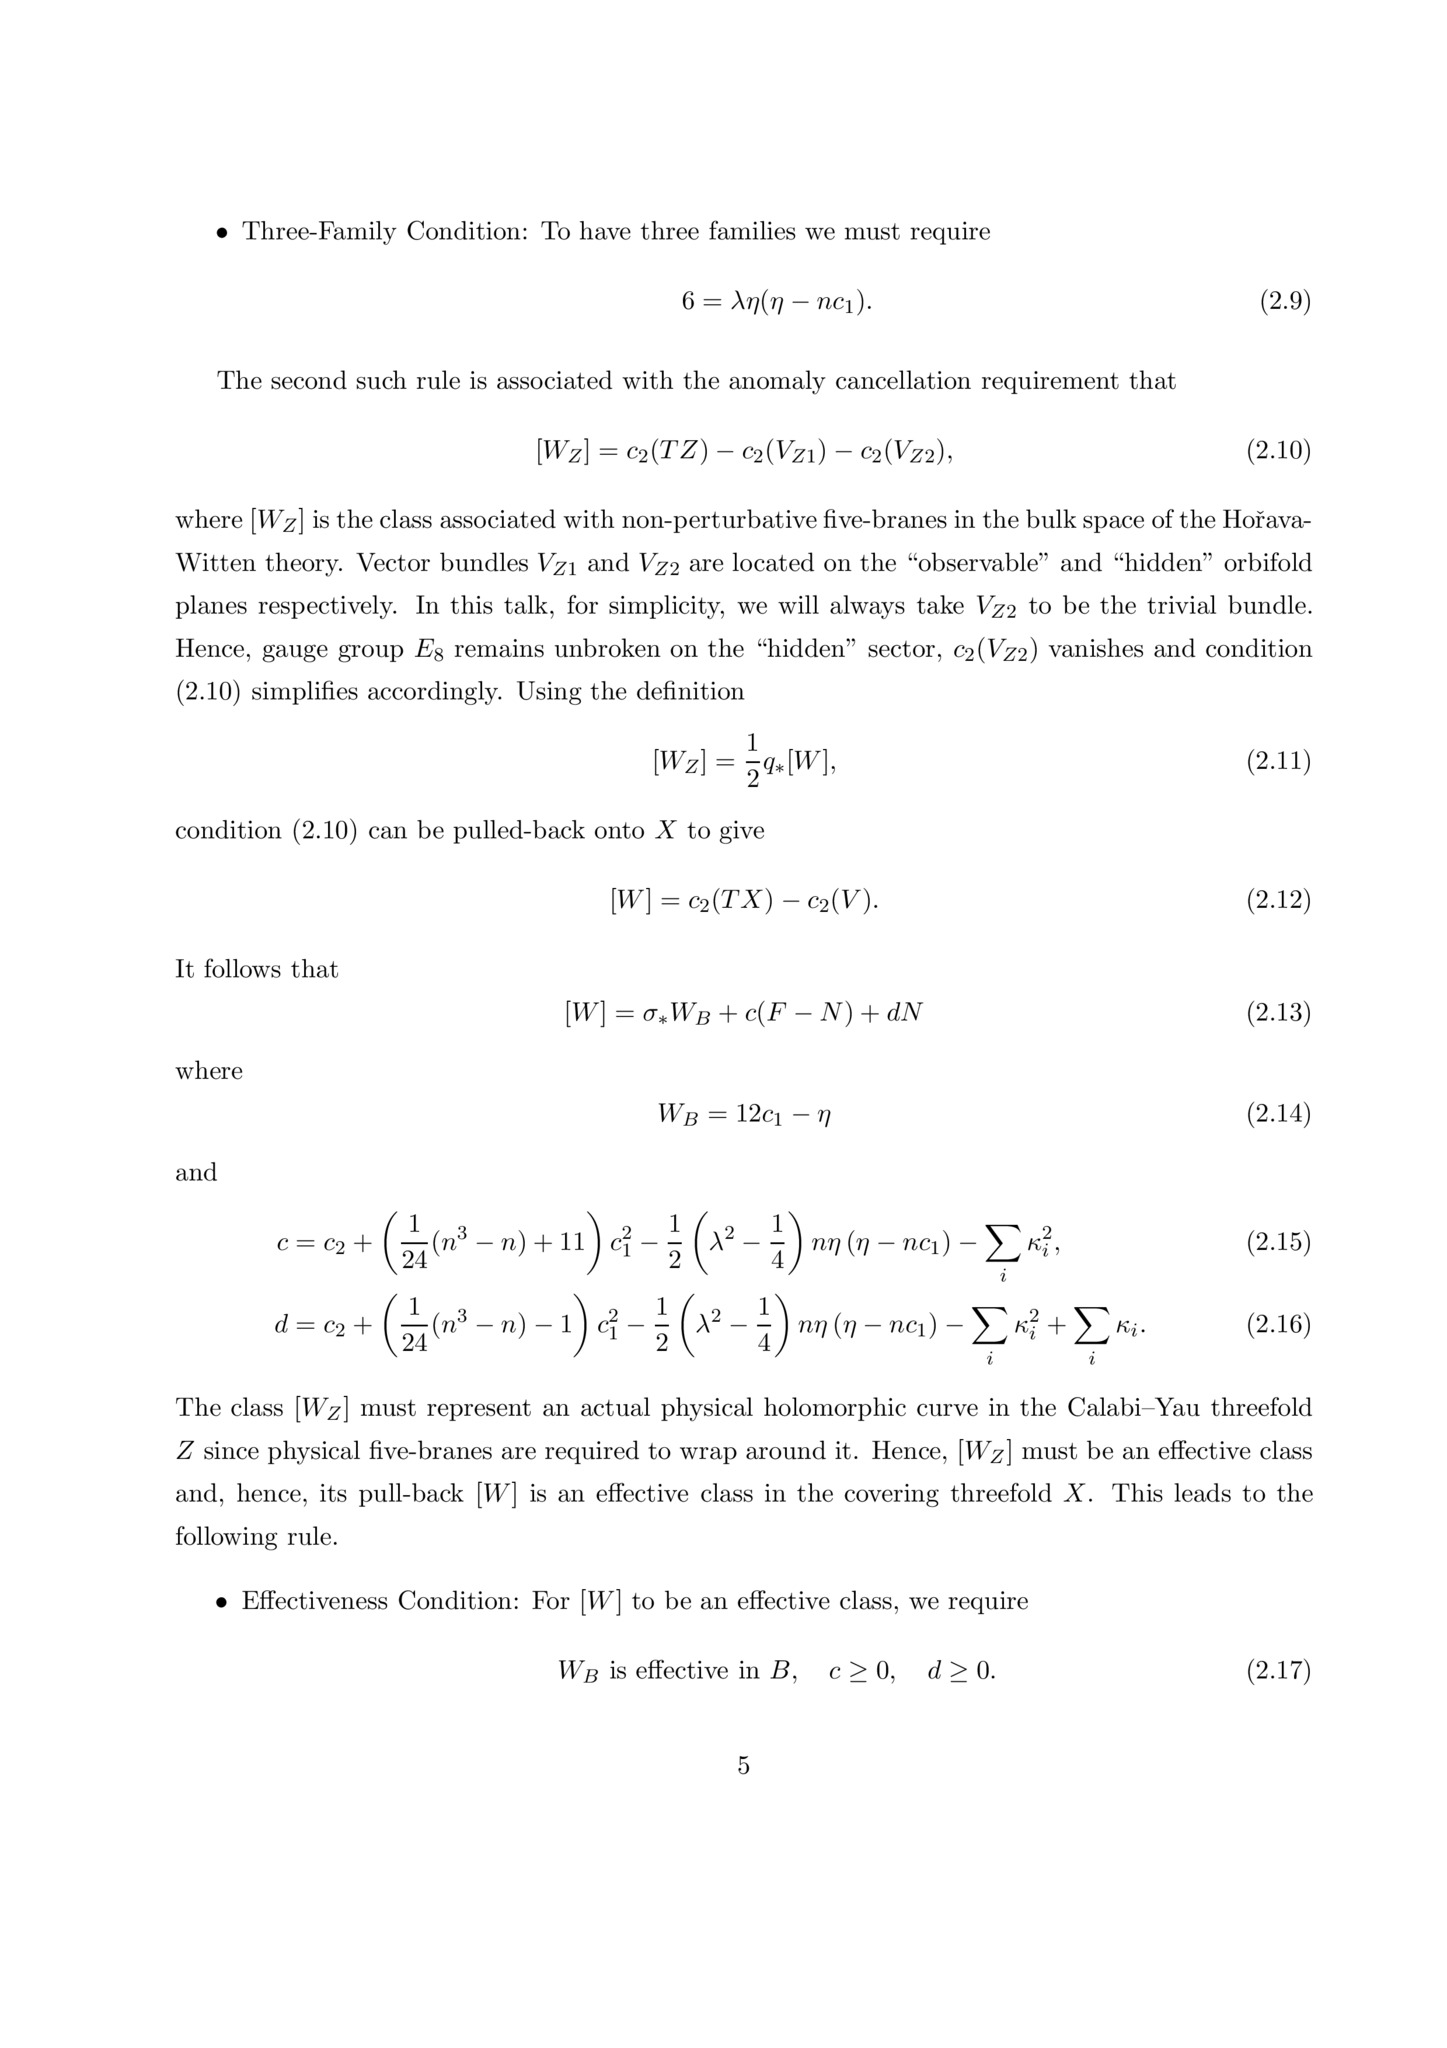
\includegraphics[scale=0.25]{img/dataset/input.jpg}
    \caption{Пример входного изображения}
    \label{dataset_input}
\end{figure}

\begin{figure}
    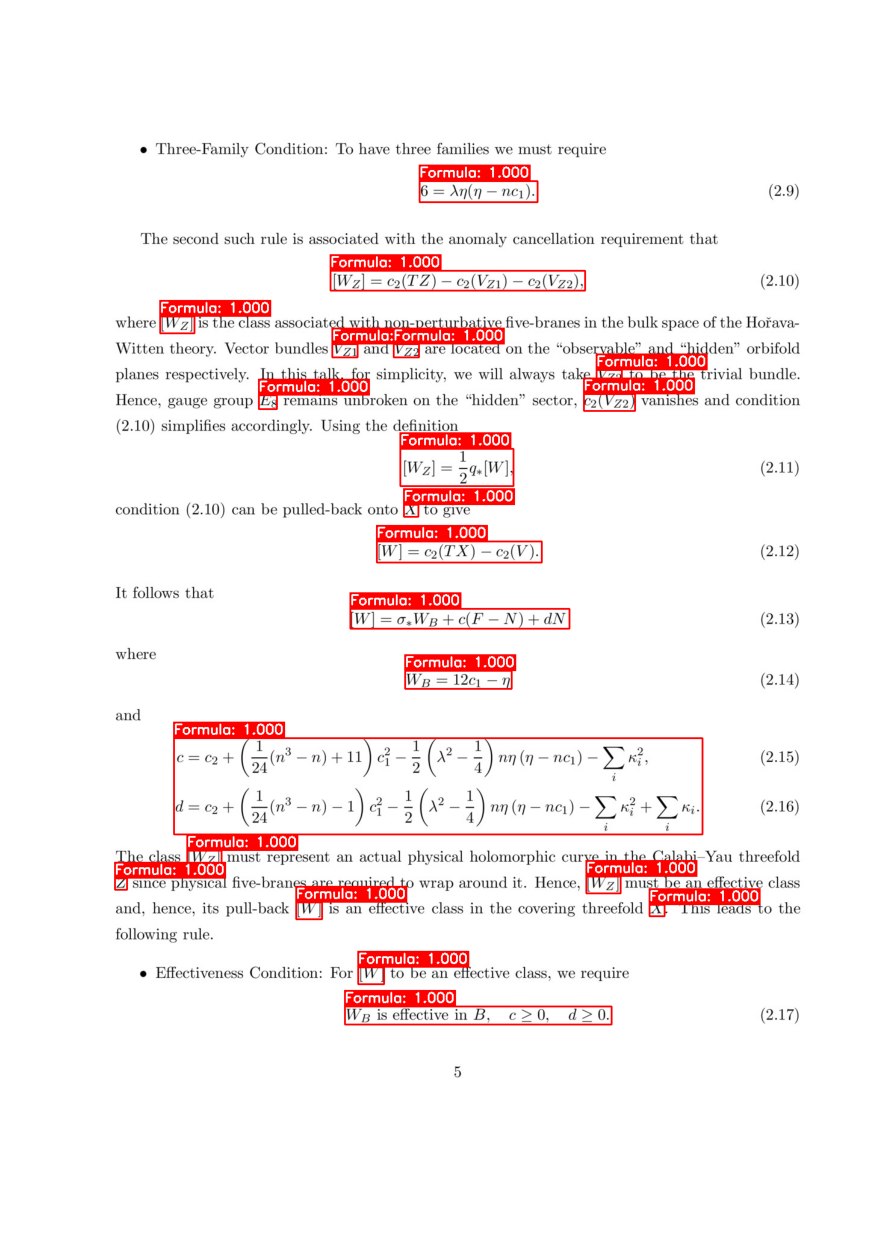
\includegraphics[scale=0.5]{img/dataset/parsed.png}
    \caption{Пример изображения с метками формул}
    \label{dataset_output}
\end{figure}

\subsubsection{Обучение}

Обучение проводилось на платформе $Kaggle$ \cite{kaggle} с логгированием в системе $wandb$ \cite{wandb}. В качестве графического процессора использовались две видеокарты $Tesla\;T4$
После обучения модели мы переходим к оценки ее эффективности. Посмотрим на полученные с помощью $wandb$ графики описанных выше метрик.
\begin{figure}
    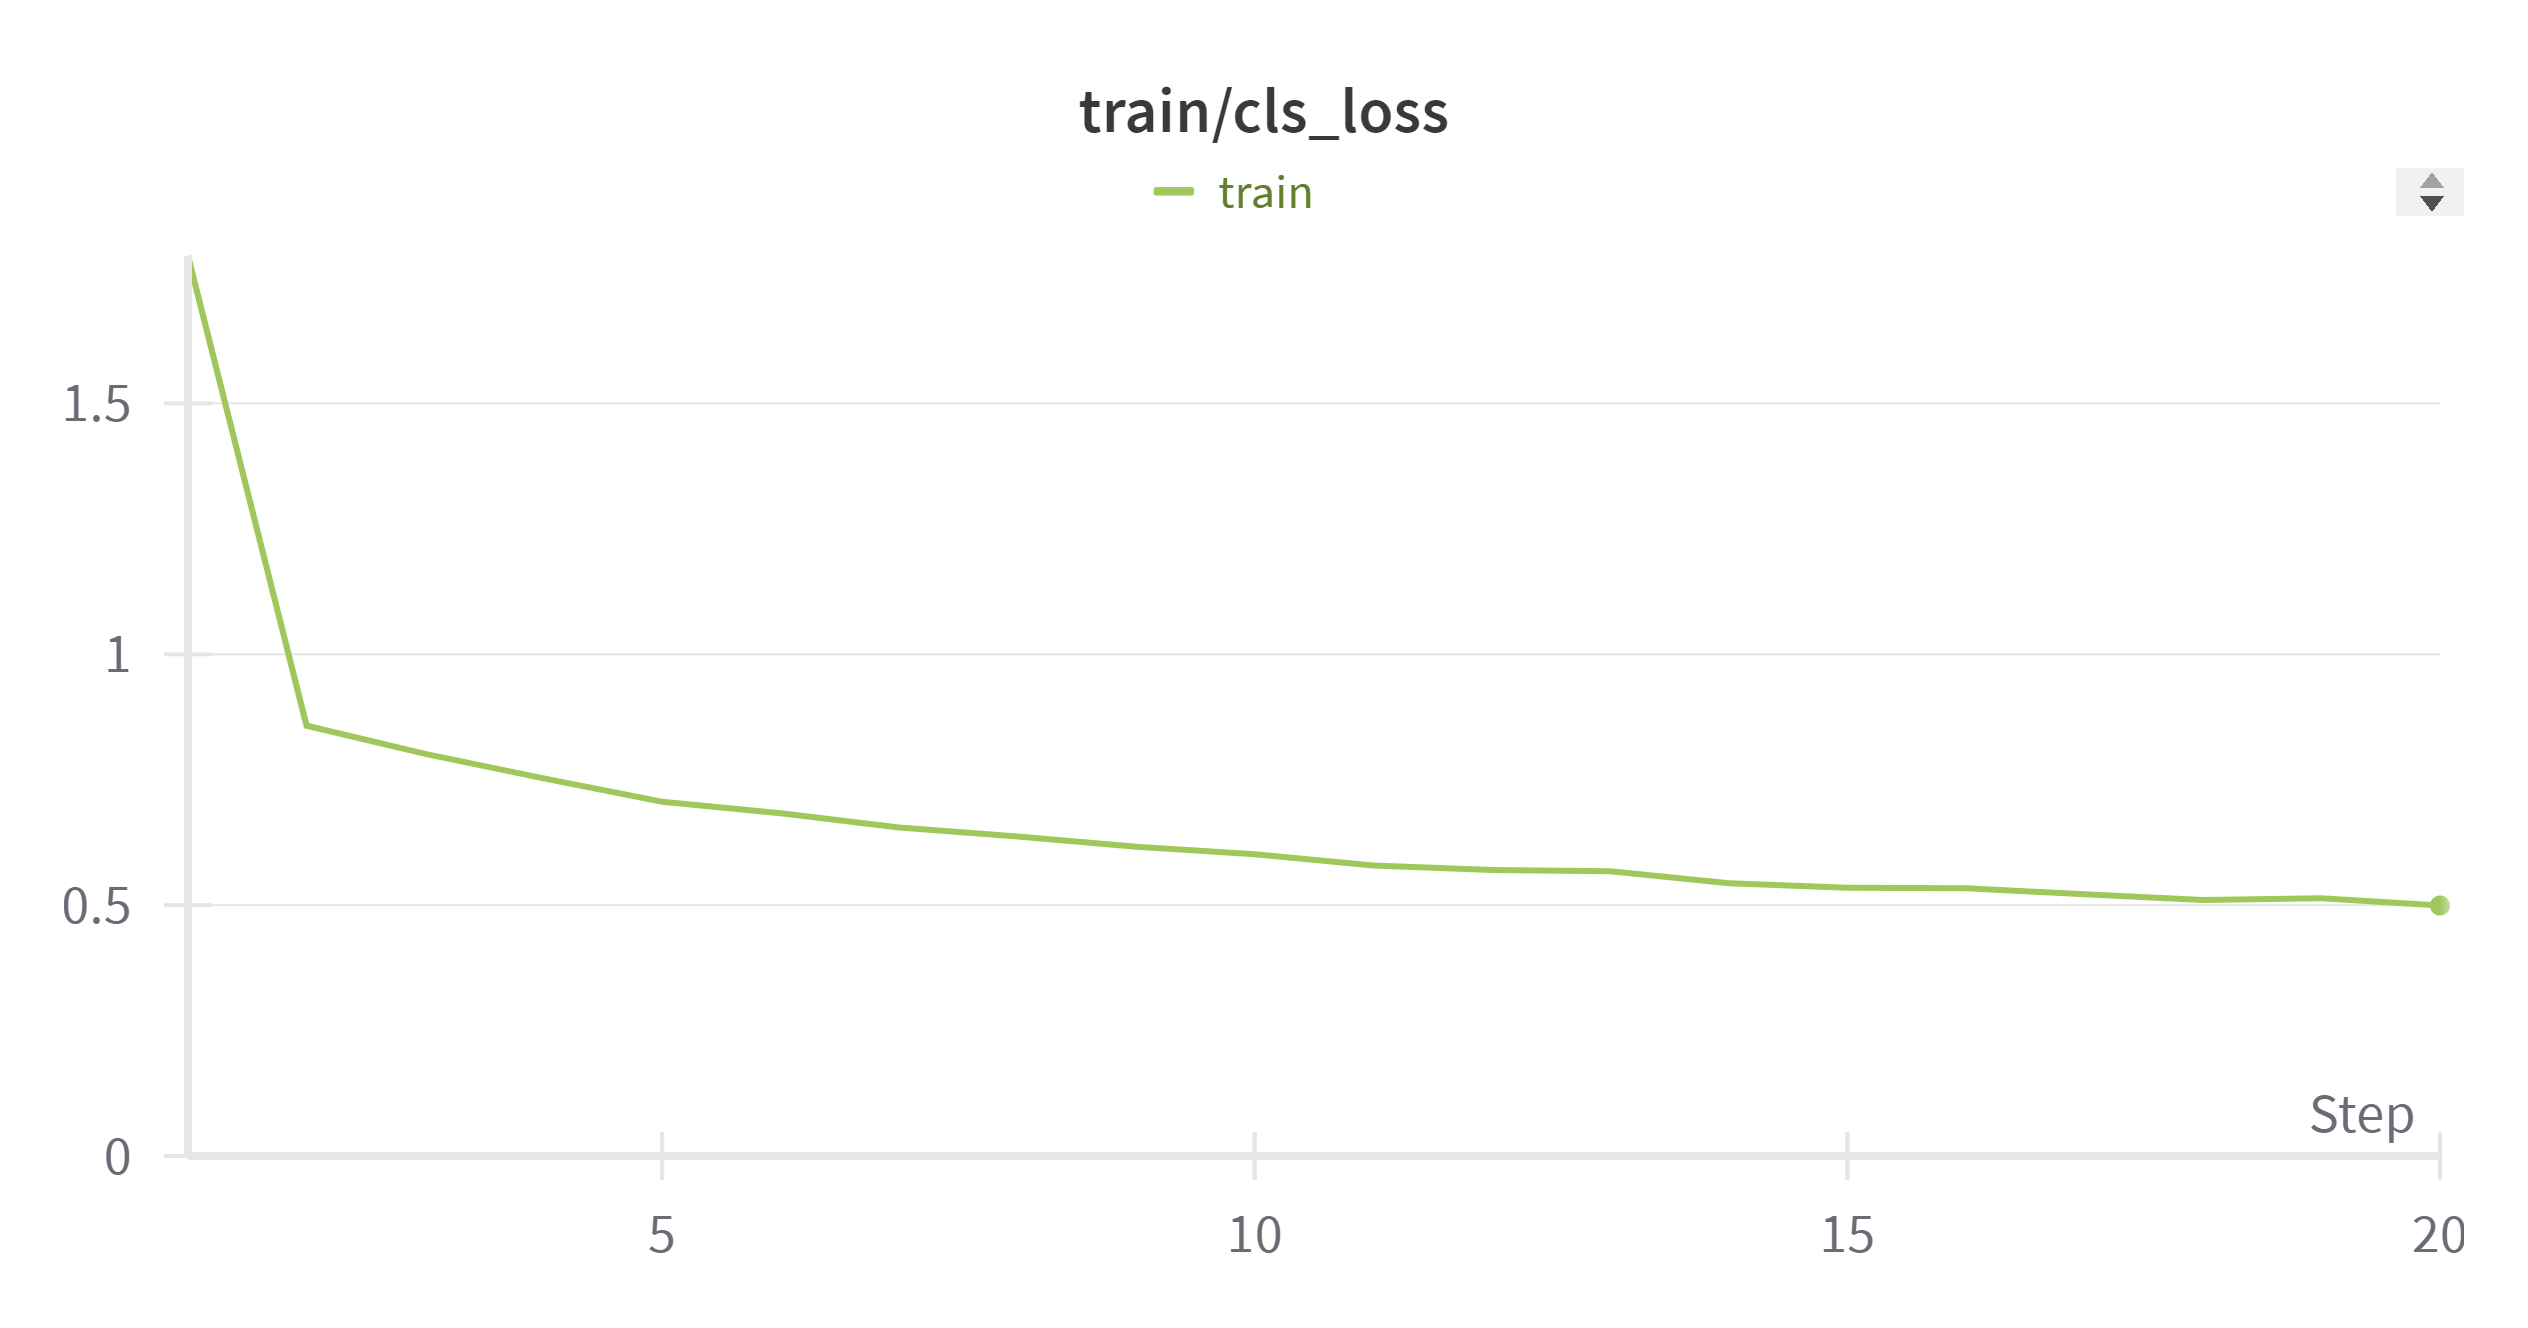
\includegraphics[scale=0.15]{img/train/train_cls_loss.png}
    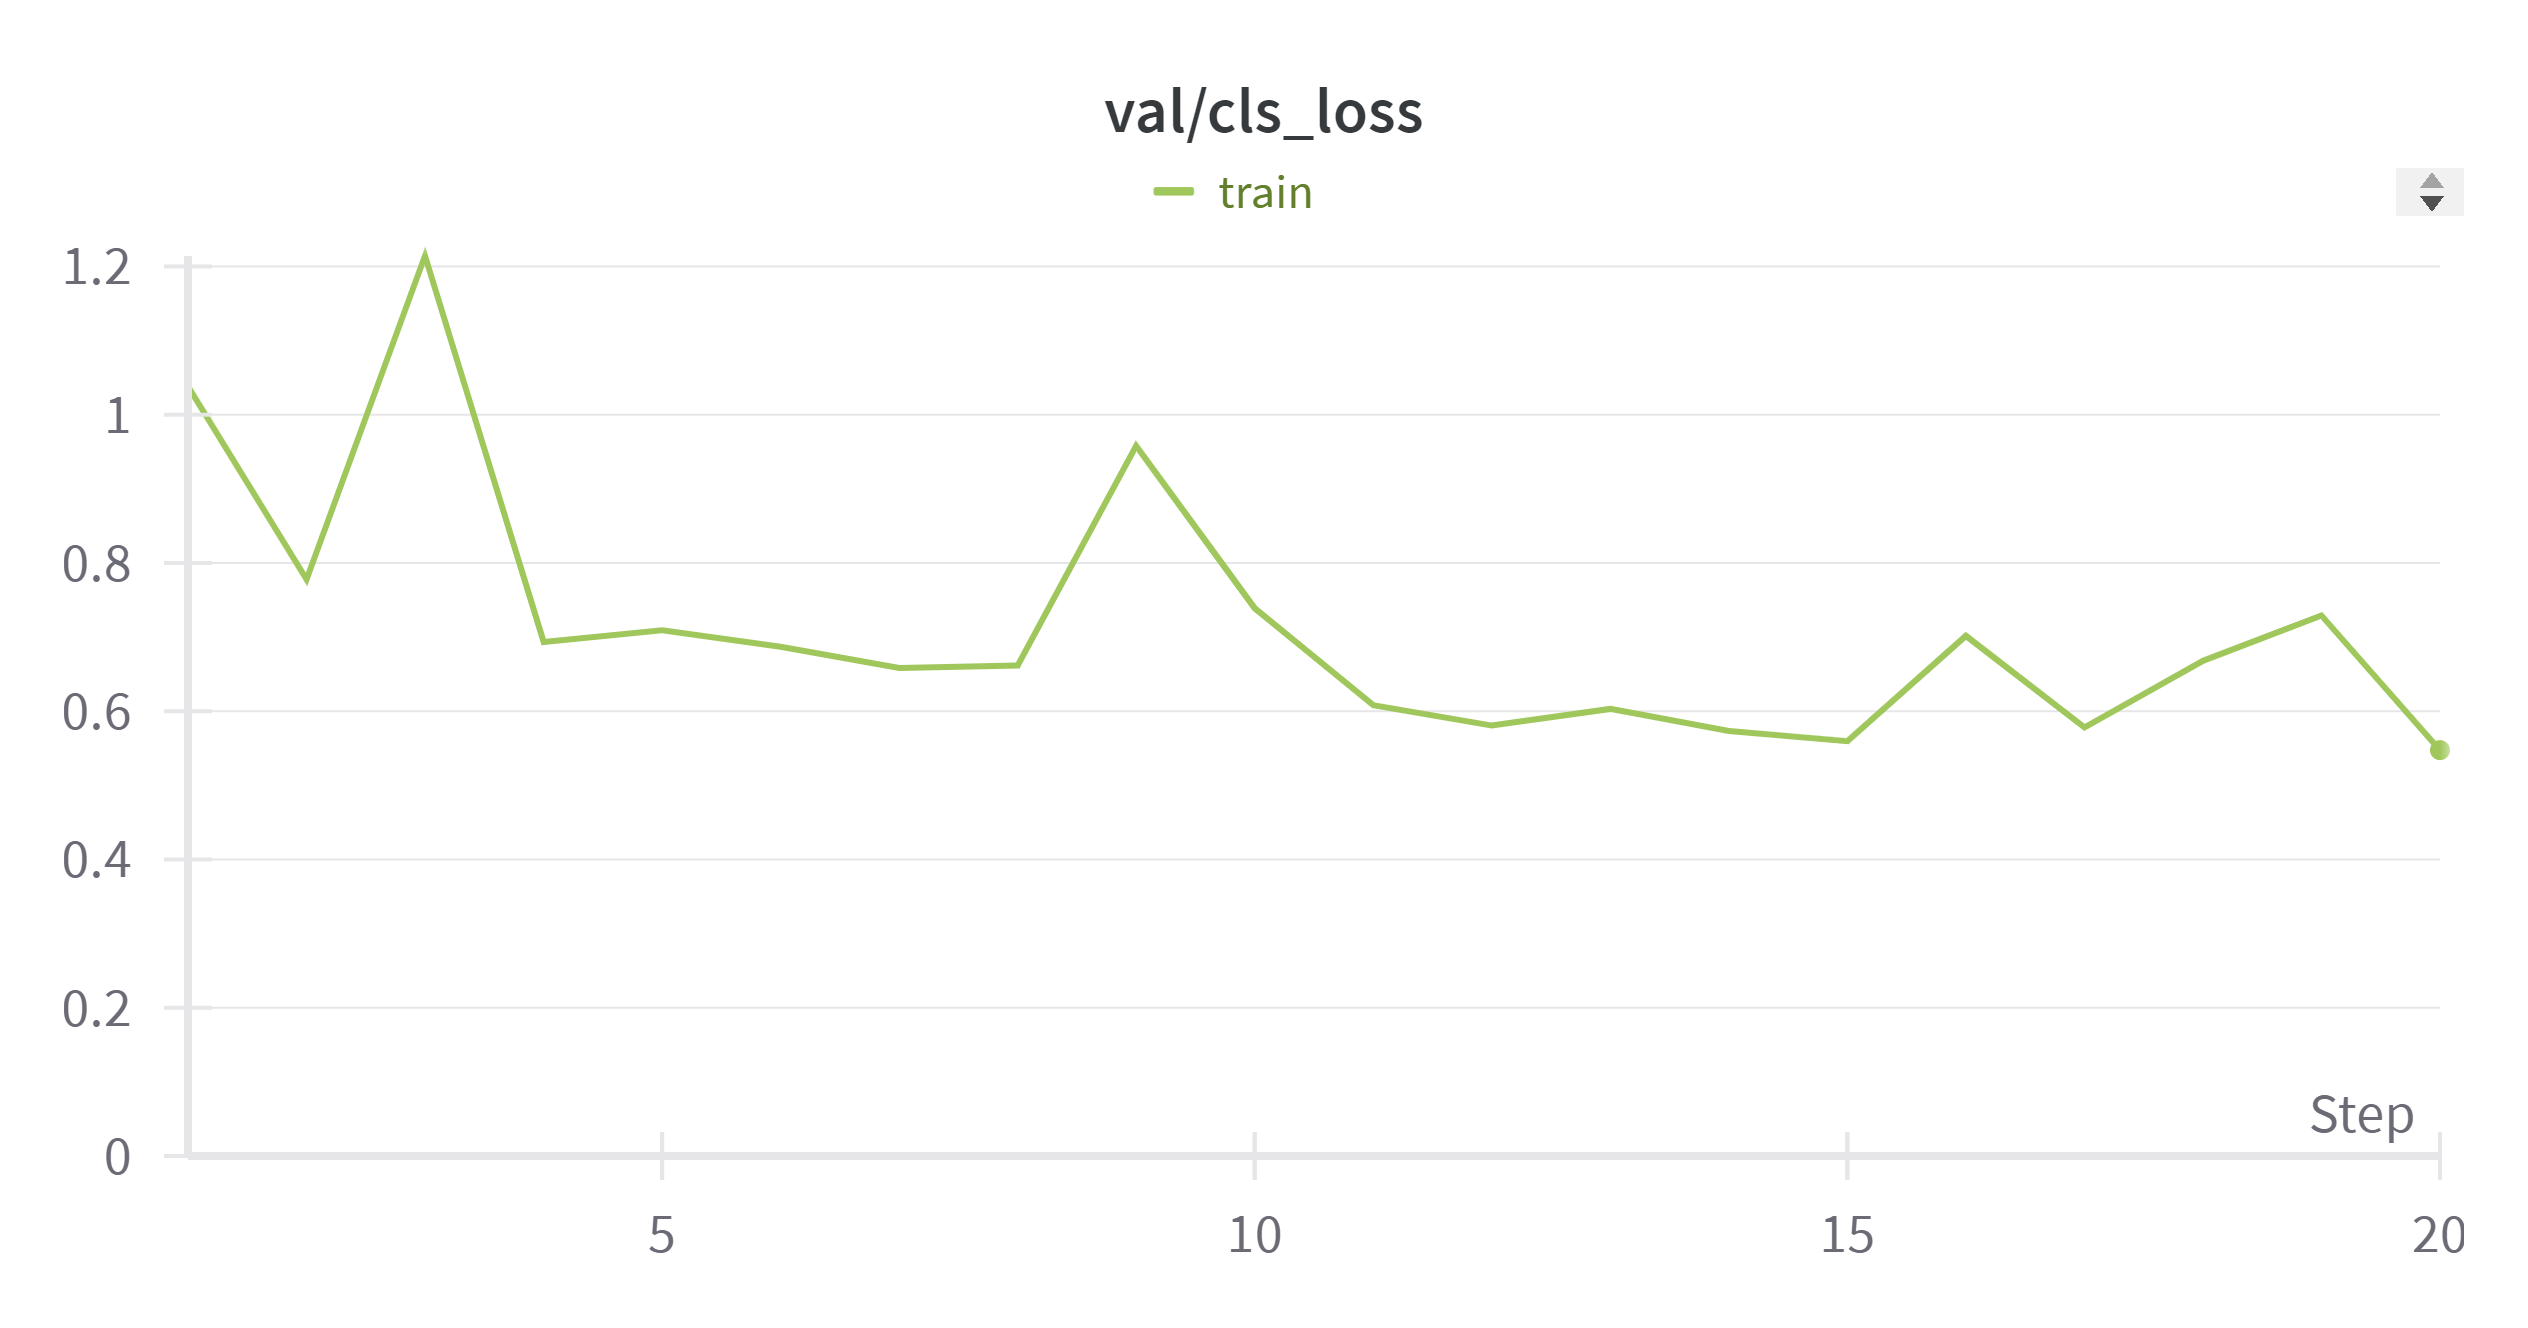
\includegraphics[scale=0.15]{img/train/val_cls_loss.png}
    \caption{Графики потерь}
    \label{cls_loss_graph}
\end{figure}

\begin{figure}
    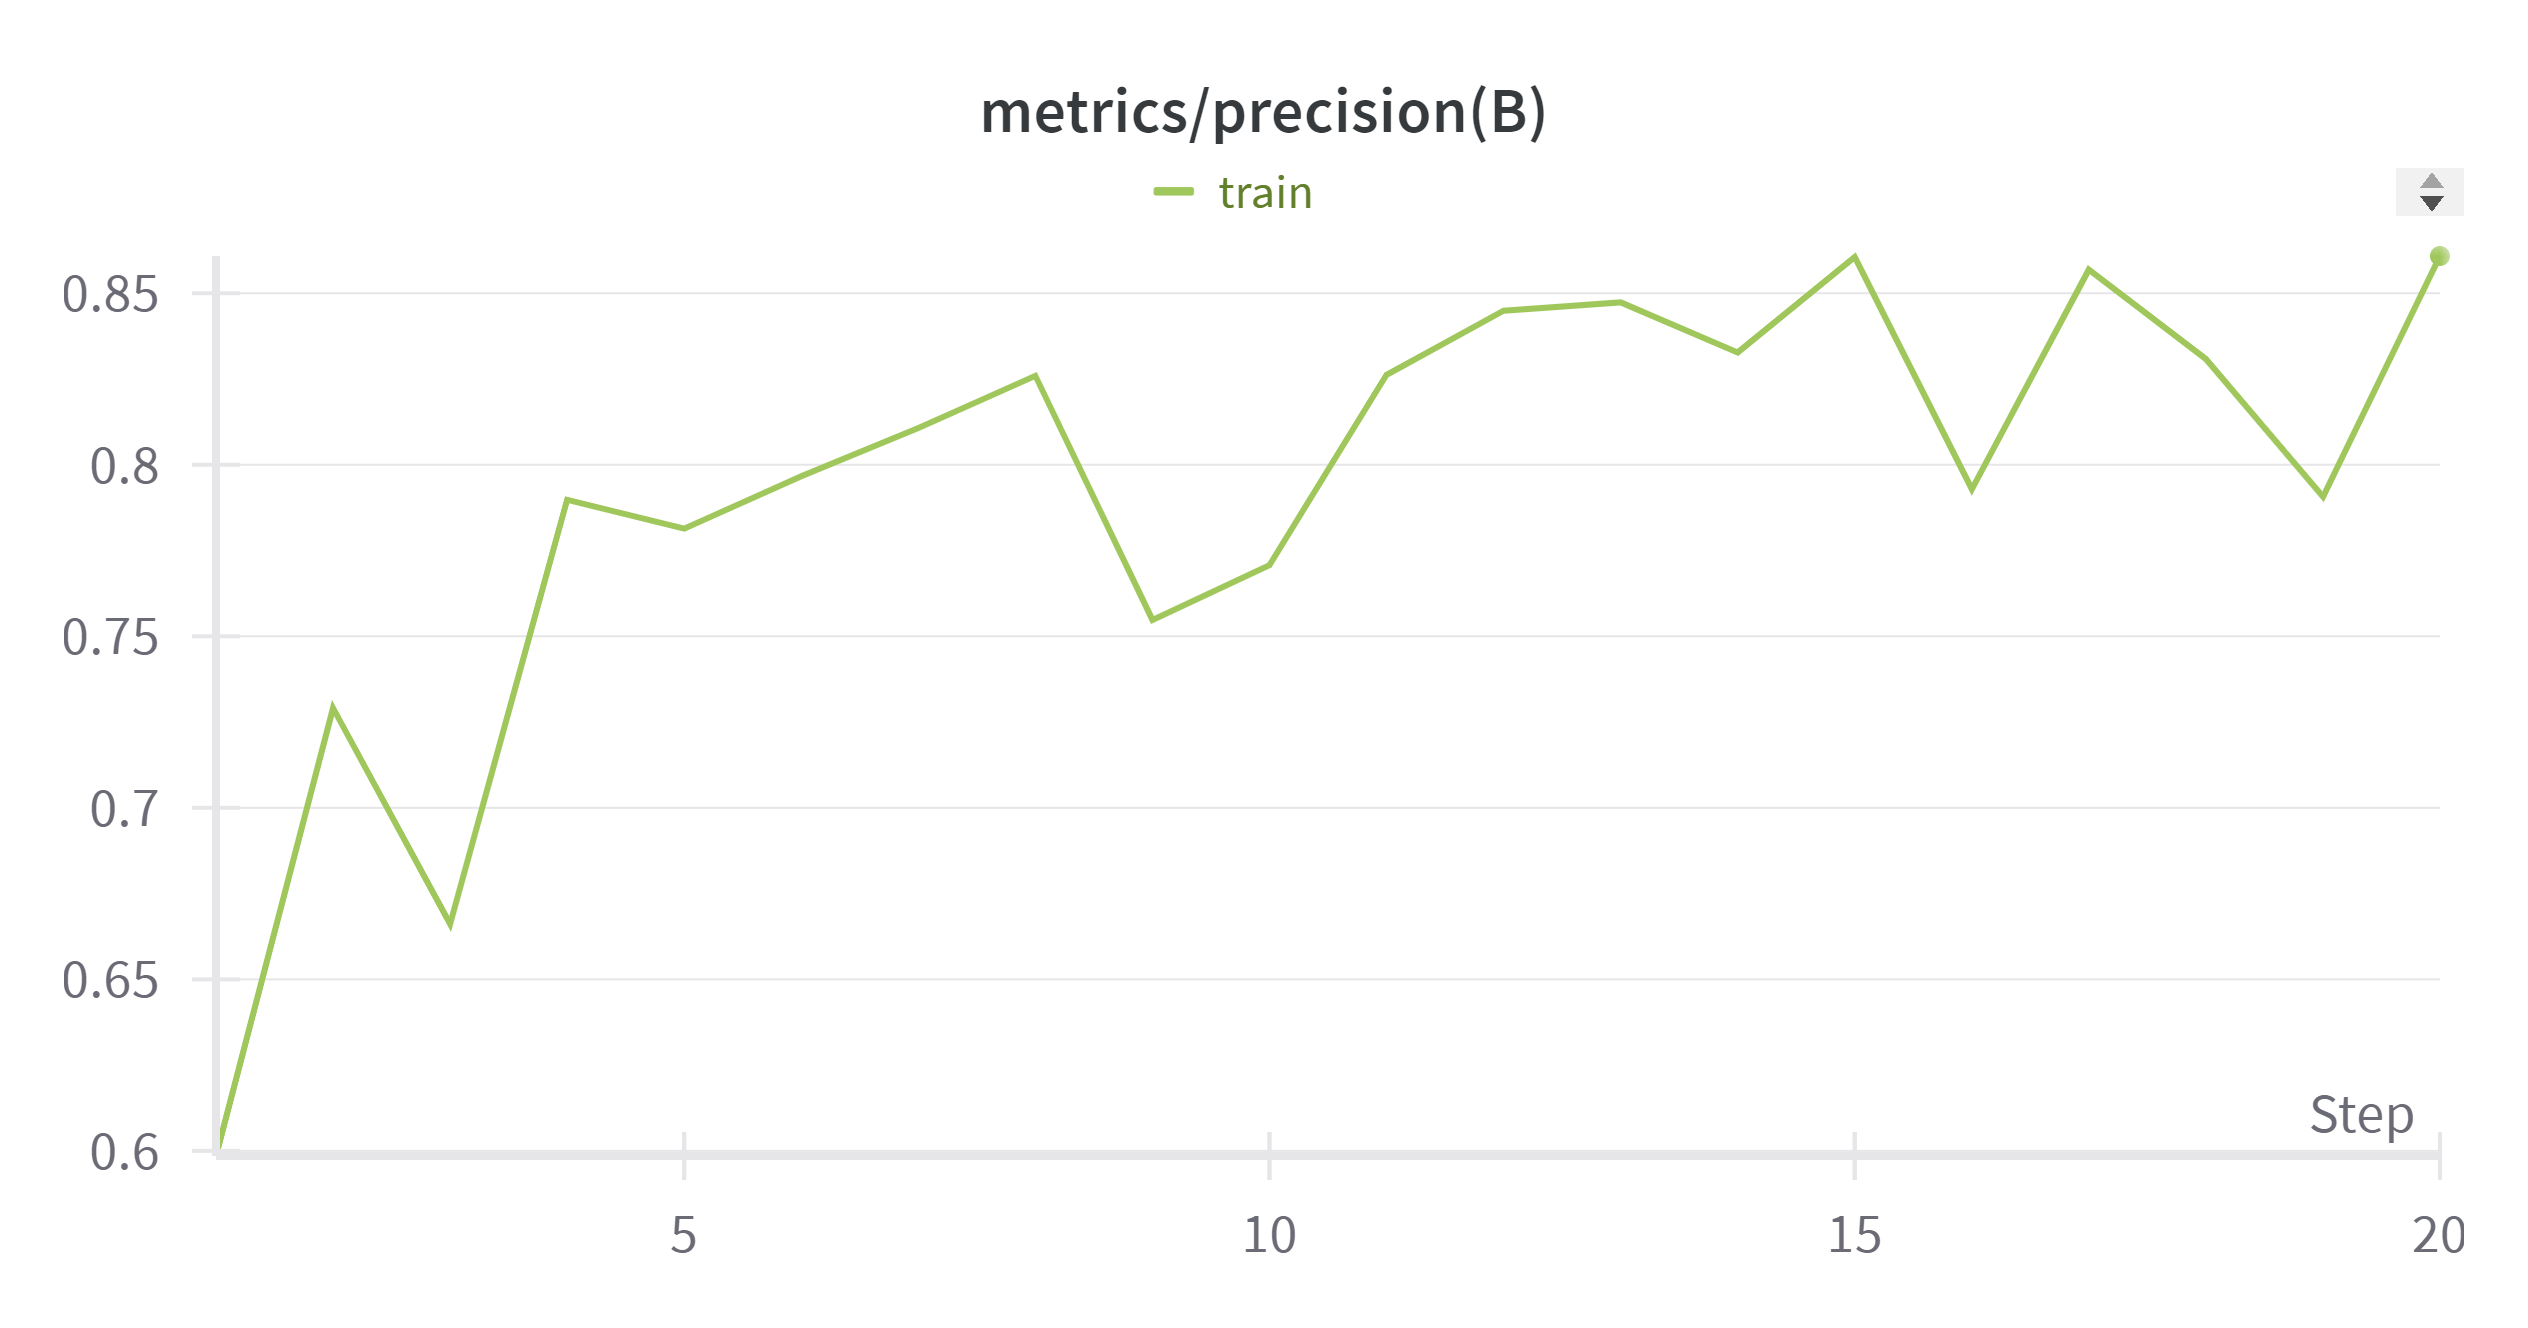
\includegraphics[scale=0.15]{img/train/precision.png}
    \caption{График точности}
    \label{precision_graph}
\end{figure}

\begin{figure}
    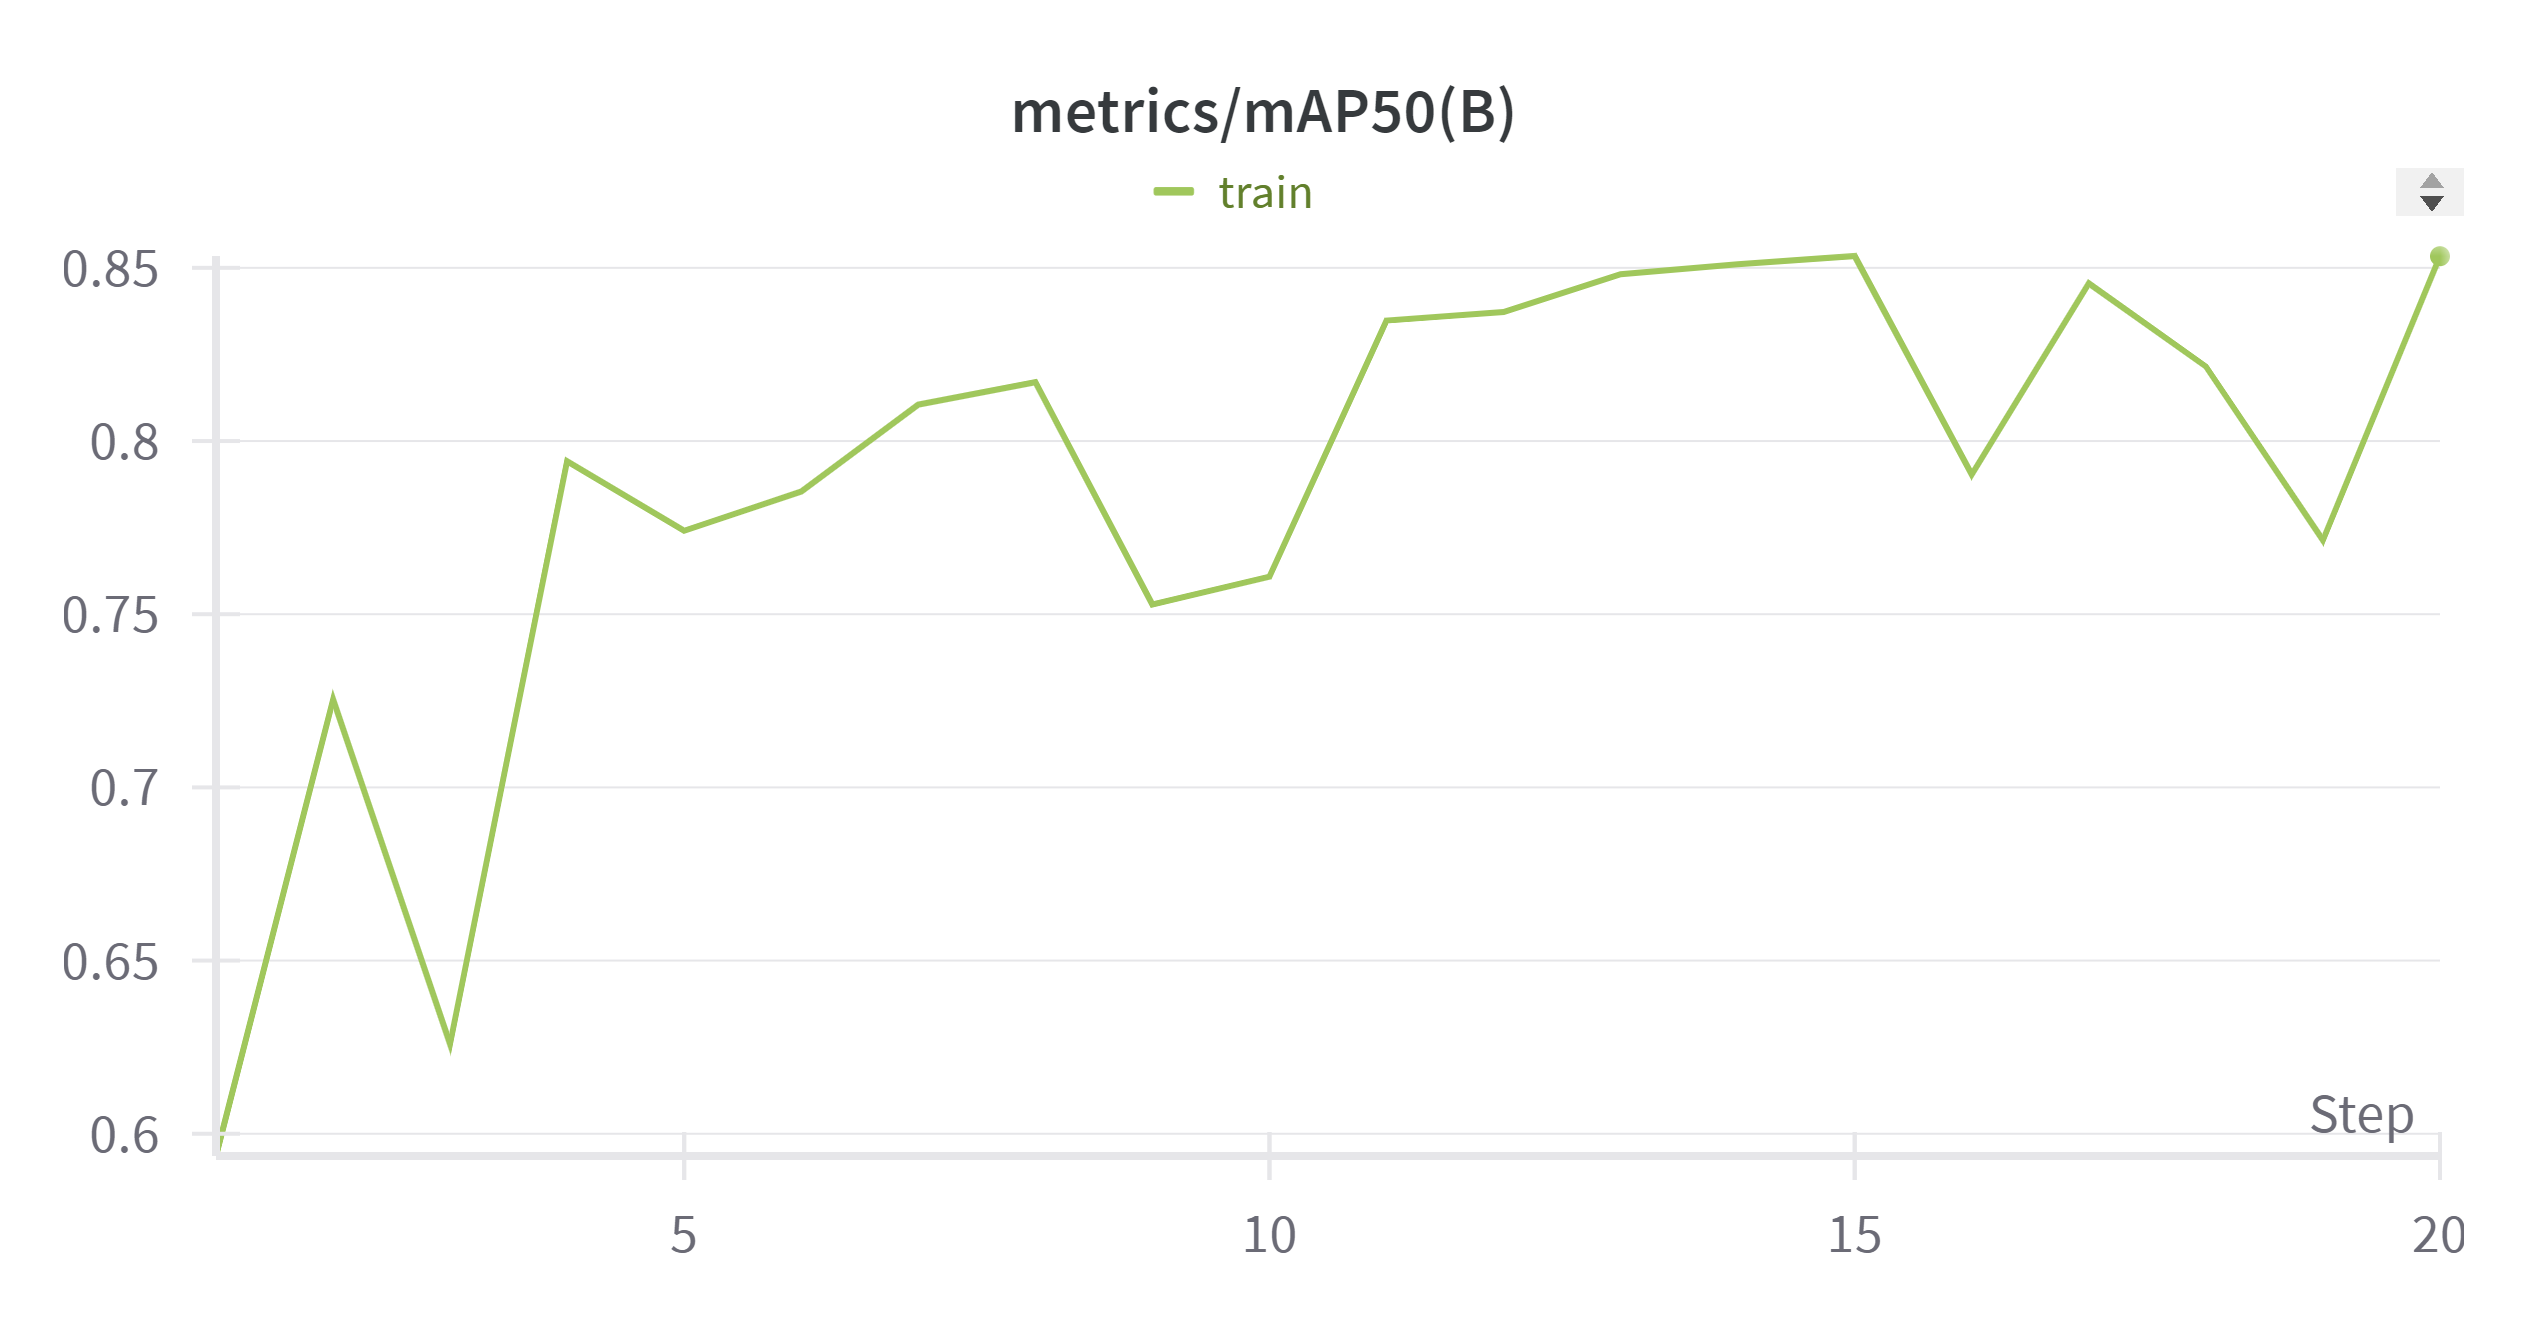
\includegraphics[scale=0.15]{img/train/map_50.png}
    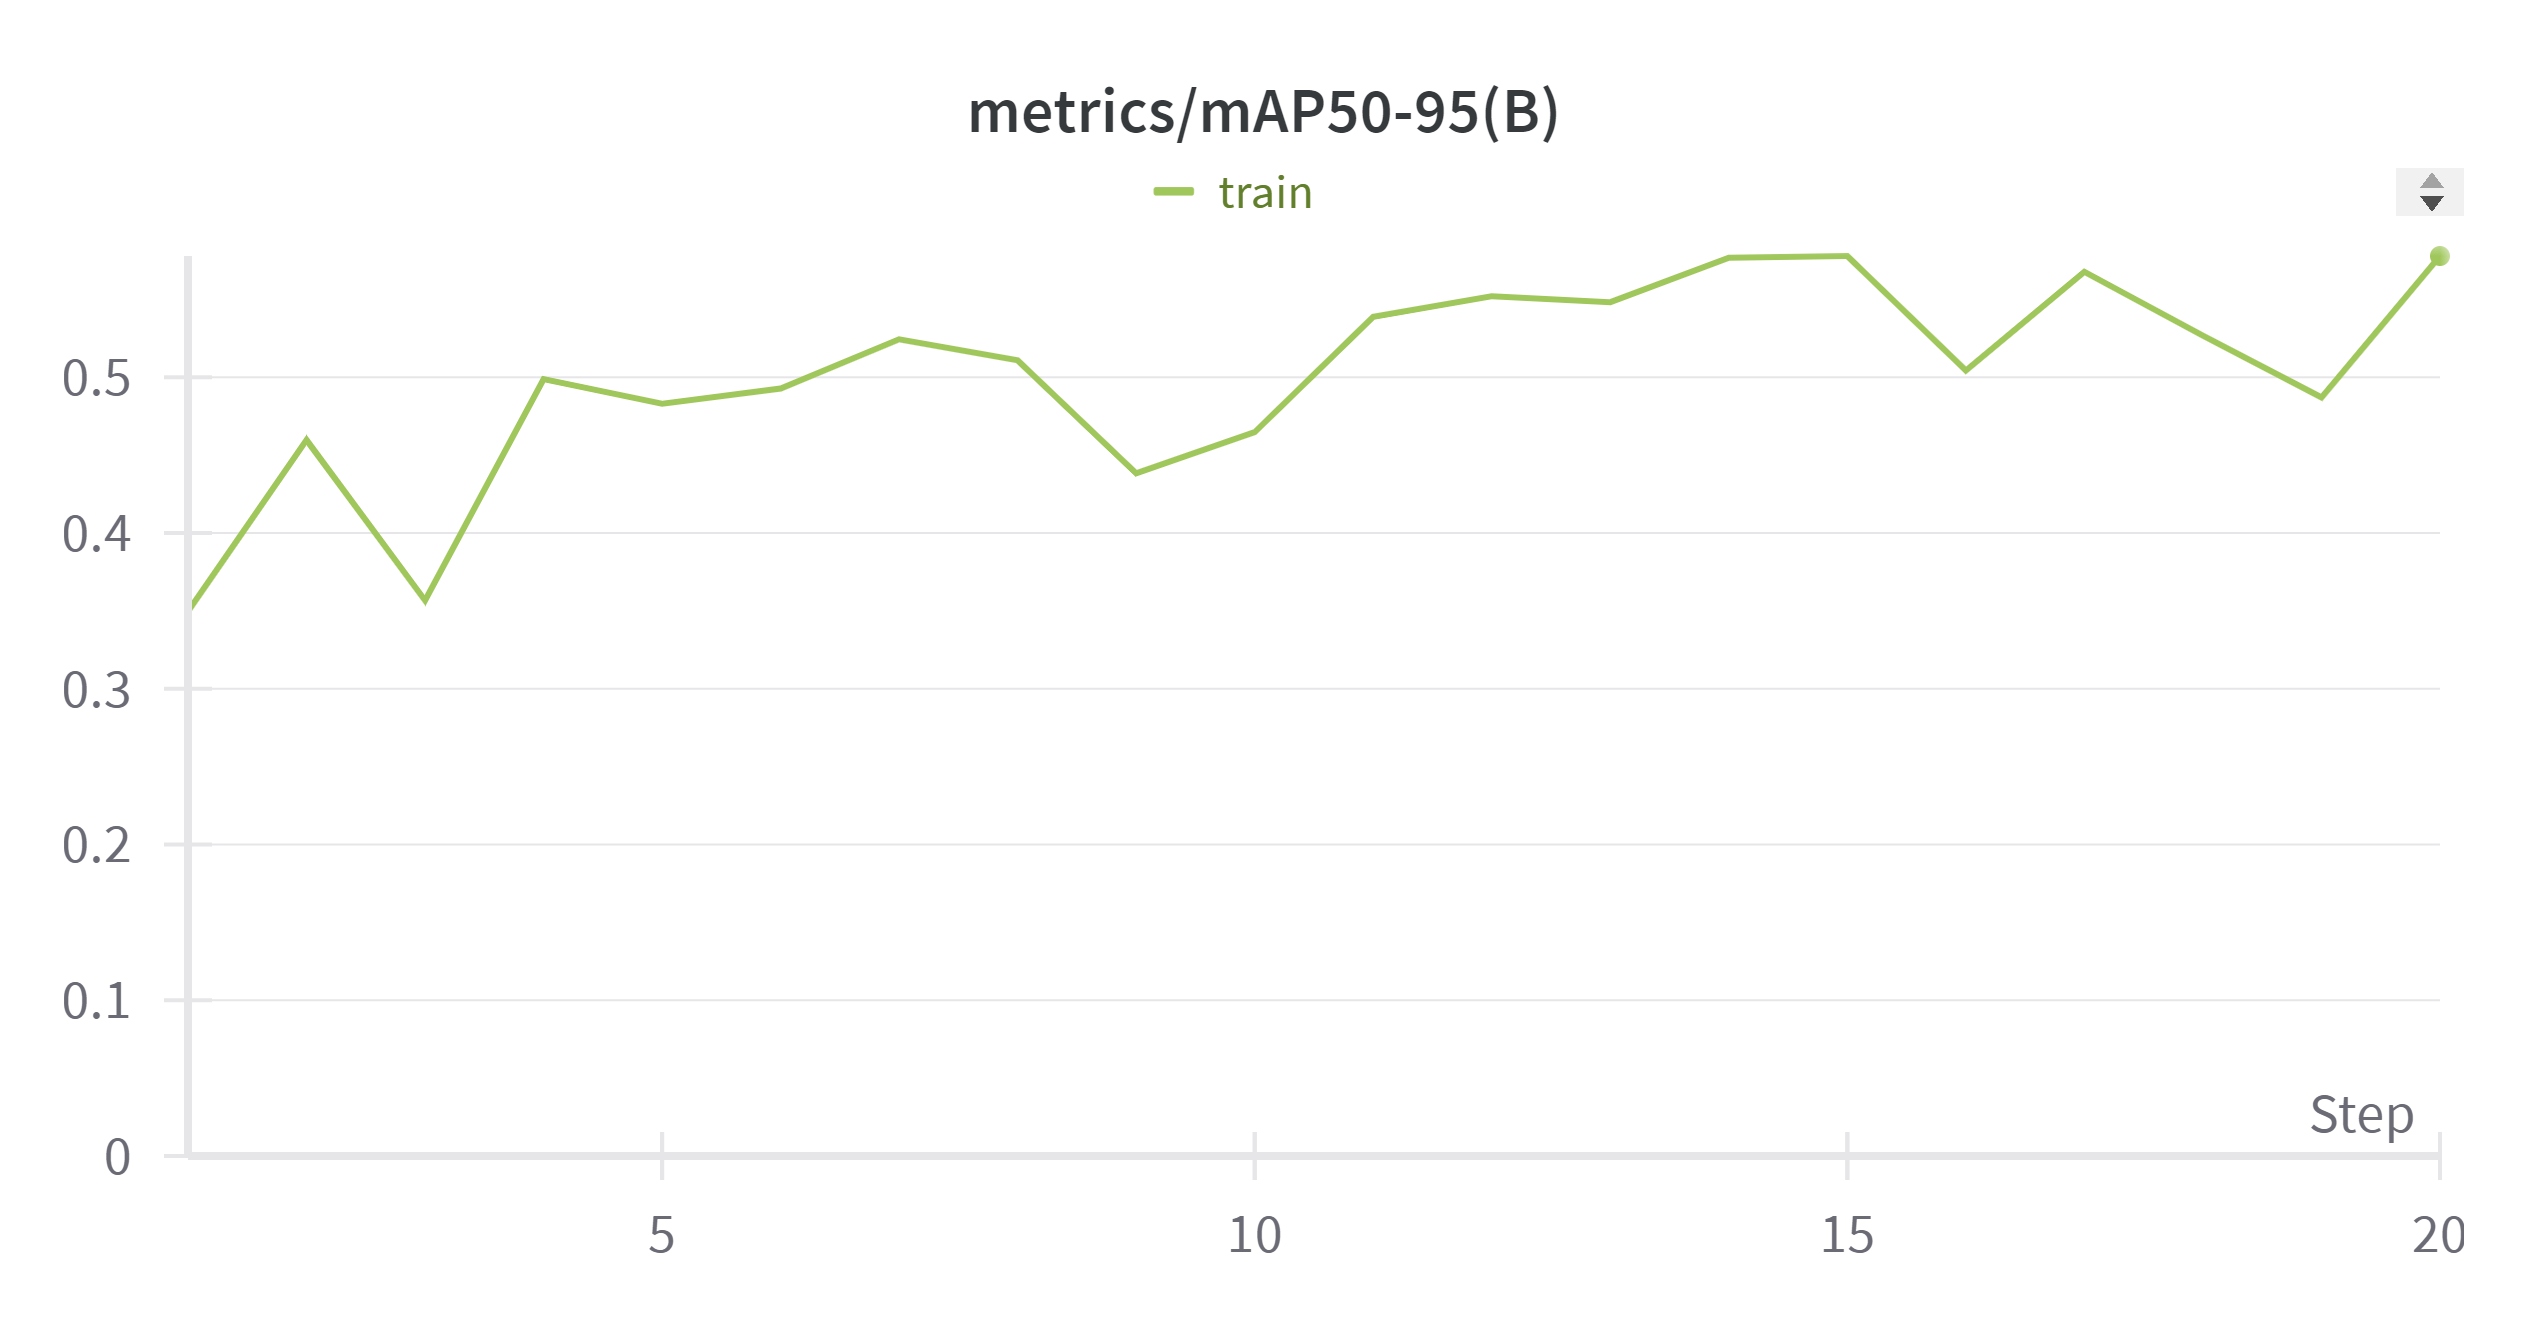
\includegraphics[scale=0.15]{img/train/map50_95.png}
    \caption{Графики $mAP$}
    \label{map_graph}
\end{figure}

На каждом из графиков ~\ref{cls_loss_graph} \dots ~\ref{map_graph} по оси $oX$ отложен номер шага, на котором снимались показатели. Весь этап обучения, состоящий из $N$ эпох равномерно делится на $20$ этапов. На каждом этапе снимаются метрики, попадающие в результирующий график.

После обучения модель была протестирована на тестовых изображениях. На рисунках ~\ref{train_test_1} и ~\ref{train_test_2} показаны результаты тестирования.

\begin{figure}
    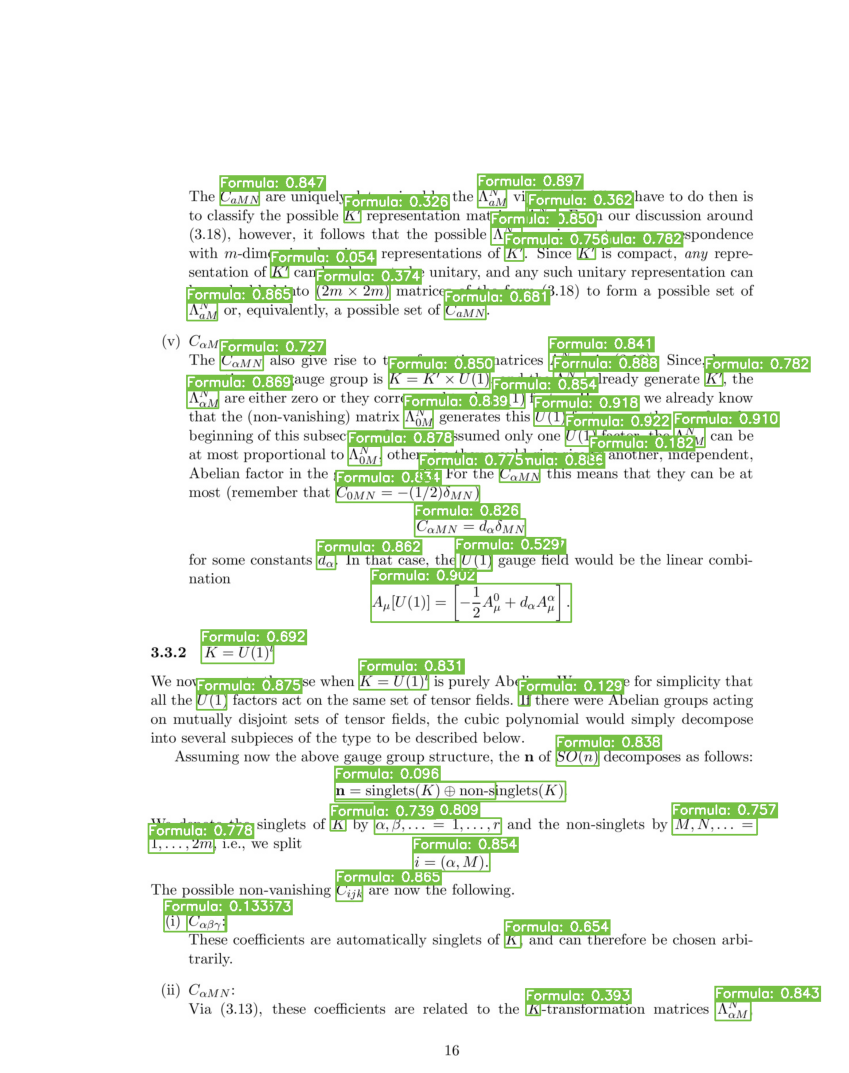
\includegraphics[scale=0.75]{img/train/test_1.png}
    \caption{Предсказание модели на тестовом изображении}
    \label{train_test_1}
\end{figure}

\begin{figure}
    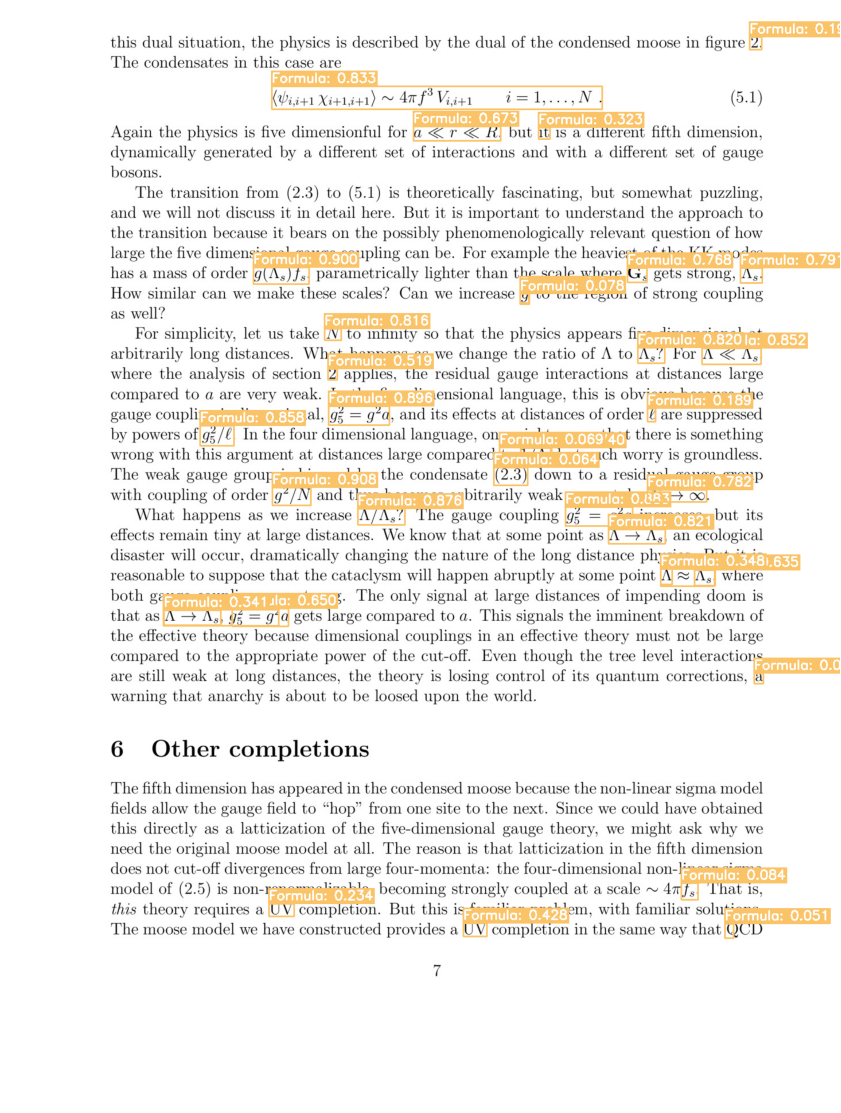
\includegraphics[scale=0.75]{img/train/test_2.png}
    \caption{Предсказание модели на тестовом изображении}
    \label{train_test_2}
\end{figure}